\documentclass[14pt,xcolor=pdftex,dvipsnames,table]{beamer}\usepackage[]{graphicx}\usepackage[]{color}
%% maxwidth is the original width if it is less than linewidth
%% otherwise use linewidth (to make sure the graphics do not exceed the margin)
\makeatletter
\def\maxwidth{ %
  \ifdim\Gin@nat@width>\linewidth
    \linewidth
  \else
    \Gin@nat@width
  \fi
}
\makeatother

\definecolor{fgcolor}{rgb}{0.345, 0.345, 0.345}
\newcommand{\hlnum}[1]{\textcolor[rgb]{0.686,0.059,0.569}{#1}}%
\newcommand{\hlstr}[1]{\textcolor[rgb]{0.192,0.494,0.8}{#1}}%
\newcommand{\hlcom}[1]{\textcolor[rgb]{0.678,0.584,0.686}{\textit{#1}}}%
\newcommand{\hlopt}[1]{\textcolor[rgb]{0,0,0}{#1}}%
\newcommand{\hlstd}[1]{\textcolor[rgb]{0.345,0.345,0.345}{#1}}%
\newcommand{\hlkwa}[1]{\textcolor[rgb]{0.161,0.373,0.58}{\textbf{#1}}}%
\newcommand{\hlkwb}[1]{\textcolor[rgb]{0.69,0.353,0.396}{#1}}%
\newcommand{\hlkwc}[1]{\textcolor[rgb]{0.333,0.667,0.333}{#1}}%
\newcommand{\hlkwd}[1]{\textcolor[rgb]{0.737,0.353,0.396}{\textbf{#1}}}%

\usepackage{framed}
\makeatletter
\newenvironment{kframe}{%
 \def\at@end@of@kframe{}%
 \ifinner\ifhmode%
  \def\at@end@of@kframe{\end{minipage}}%
  \begin{minipage}{\columnwidth}%
 \fi\fi%
 \def\FrameCommand##1{\hskip\@totalleftmargin \hskip-\fboxsep
 \colorbox{shadecolor}{##1}\hskip-\fboxsep
     % There is no \\@totalrightmargin, so:
     \hskip-\linewidth \hskip-\@totalleftmargin \hskip\columnwidth}%
 \MakeFramed {\advance\hsize-\width
   \@totalleftmargin\z@ \linewidth\hsize
   \@setminipage}}%
 {\par\unskip\endMakeFramed%
 \at@end@of@kframe}
\makeatother

\definecolor{shadecolor}{rgb}{.97, .97, .97}
\definecolor{messagecolor}{rgb}{0, 0, 0}
\definecolor{warningcolor}{rgb}{1, 0, 1}
\definecolor{errorcolor}{rgb}{1, 0, 0}
\newenvironment{knitrout}{}{} % an empty environment to be redefined in TeX

\usepackage{alltt}

% Specify theme
\usetheme{Madrid}
% See deic.uab.es/~iblanes/beamer_gallery/index_by_theme.html for other themes
\usepackage{caption}
\usepackage{tikz}
\usetikzlibrary{calc,matrix}
\usepackage{multirow}
% Specify base color
\usecolortheme[named=OliveGreen]{structure}
% See http://goo.gl/p0Phn for other colors

% Specify other colors and options as required
\setbeamercolor{alerted text}{fg=Maroon}
\setbeamertemplate{items}[square]

% Title and author information
\title{Oligopoly}
\author{Rob Hayward}
\IfFileExists{upquote.sty}{\usepackage{upquote}}{}
\begin{document}

\begin{frame}
\titlepage
\end{frame}


\section{Imperfect Competition}
\begin{frame}{Imperfect competition}
There are two broad categories of \emph{imperfect competition} 
\pause
\begin{itemize}[<+-| alert@+>]
\item Monopolistic competition:  where there is \emph{product differentiation}.  There tend to be lots of small companies because there are no barriers to entry
\item Oligopoly:  where there is price discrimination and some barriers to entry. There tend to be a few large companies
\end{itemize}
\end{frame}


\begin{frame}{Competition vs monopoly}
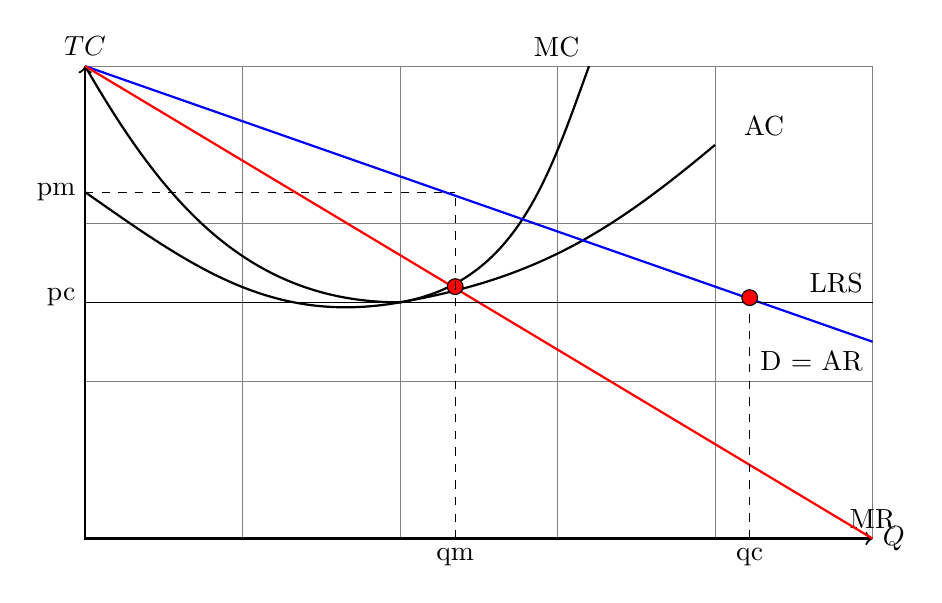
\begin{tikzpicture}[scale = 2]
\draw[very thin, color = gray] (0, 0) grid (5, 3);
\draw [<->, thick] (0, 3) node (yaxis) [above] {$TC$} 
  |- (5, 0) node (xaxis) [right] {$Q$};
\node at (4.5, 2.5) [above left] {AC};
\node at (3.2, 3) [above left] {MC};
\draw [thick] (0.0, 3.0) to [out = -60, in = 180] (2, 1.5) to 
[out = 10, in = 220] (4, 2.5);
\draw [thick] (0, 2.2) to [out = -35, in = 190] (2, 1.5) to [out = 10, in = 250] (3.2, 3);
\draw [thick, color = blue] (0, 3) to (5, 1.25); 
\node at (5, 1.25) [below left] {D = AR};
\node at (5, 0) [above] {MR};
\draw [thick, color = red] (0, 3) to (5, 0);
\pause
\draw [fill = red] (2.35, 1.6) circle [radius = 0.05];
\draw [dashed] (2.35, 0) to (2.35, 2.2);
\node at (2.35, 0) [below] {qm};
\draw [dashed] (0, 2.2) to (2.35, 2.2);
\node at (0, 2.2) [left] {pm};
\pause
\draw (0, 1.5) to (5, 1.5);
\node at (5, 1.5) [above left] {LRS};
\pause
\draw [dashed] (4.22, 1.53) to (4.22, 0);
\node at (4.22, 0) [below] {qc};
\node at (0, 1.53) [left] {pc};
\draw [fill = red] (4.22, 1.53) circle [radius = 0.05];
\end{tikzpicture}
\end{frame}


\begin{frame}{Factors that influence level of competition}
The level of competition is influenced by 
\pause
\begin{itemize}[<+-| alert@+>]
\item The number of firms
\item The variability of demand
\item Changes in technology 
\item Social cohesion
\item 
\end{itemize}
\end{frame}


\section{Cartels}
\begin{frame}{Interdependence}
\begin{itemize}[<+-| alert@+>]
\item A key feature of oligopoly is \emph{interdependence}.  
\item The firm is influenced by the other firms in the industry
\item Actions (pricing and output) will depend on expected action of other firms
\item More complicated analysis.
\item Use of \emph{game theory}
\end{itemize}
\end{frame}

\begin{frame}{Duopoly}
\begin{columns}[T]
\begin{column}{.48\textwidth}
\begin{center}
\rowcolors{1}{OliveGreen!20}{OliveGreen!5}
\begin{tabular}{r r r}
Q & P & TR (P $\times$ Q\\
\hline
0 & 120 & 0\\
20 & 100 & 2000\\
40 & 80 & 3200\\
60 & 60 & 3600\\
80 & 40 & 3200\\
100 & 20 & 2000\\
120 & 0 & 0\\
\end{tabular}
\end{center} 
\end{column}
\begin{column}{.48\textwidth}
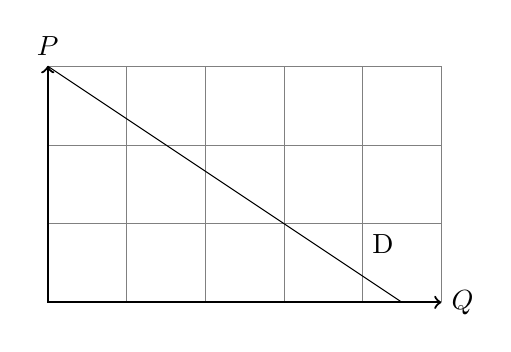
\begin{tikzpicture}
\draw[very thin, color = gray](0, 0) grid (5, 3);
\draw [<->, thick] (0, 3) node (yaxis) [above] {$P$} 
  |- (5, 0) node (xaxis) [right] {$Q$};
\node at (4, 0.5) [above right] {D};
\draw (0, 3) to (4.5, 0);
%\draw (0.25, 0.25) to (4.5, 3);
%\draw [dashed] (5, 1.70) to (0, 1.70);
%\draw[domain = 0.1:3.9, color = blue] plot(\x, {2 - 0.5*\x});
\end{tikzpicture}
\end{column}
\end{columns}
\end{frame}

\begin{frame}{Duopoly 2}
Outcome depends on the action of the two firms. Marginal cost of drawing water is zero
\pause
\begin{itemize}[<+-| alert@+>]
\item Competition
\begin{itemize} 
\item MC = MR = 0 (output equal to 60 litres)
\item Total output is equal to 120 litres
\end{itemize}
\item Collusion
\begin{itemize}
\item Profit is maximised at 60 litres (30 each)
\item profit is 3600 (1800 each) 
\end{itemize}
\end{itemize}

\end{frame}

\begin{frame}{Cartels}
Cartels
\begin{itemize}[<+-| alert@+>]
\item OPEC
\item LCD display 
\item England football shirts
\item FX fixing
\end{itemize}
\end{frame}

\begin{frame}{Nash equilibrium}
Without a cartel, there is an incentive to push output above the \emph{joint} profit-maximising
\pause
\begin{itemize}[<+-| alert@+>]
\item Each produce 30 litres at 60 (profit is 3600 or 1800 each)
\item There is an incentive for one to cheat and produce 40 litres
\item Total output of 70, price 50, profit 3500 (2000-1500 split)
\item Or, total output 80, price 40, profit 3200 (1600 each)
\item \emph{Nash equilibrium}
\item total output 90, price 30, profit 2700 (1500 1200 split) 
\end{itemize}
\end{frame}

\begin{frame}{Number of firms}
The larger the number of firms, the more likely that the firm will increase output.  Decision for each firm is a balance of 
\pause
\begin{itemize}[<+-| alert@+>]
\item Output effect (if price is above marginal cost, selling more will raise profit)
\item Price effect (raising output will increase total output and reduce the price and the profit on all the units sold)
\end{itemize}
\pause
At the extreme as number of firms tends to infinity, output effect dominates and there is perfect competition. 
\end{frame}


\section{Game Theory}
%\begin{frame}{Game theory}
%Game theory is the study of decision-making under interdependence. 
%\pause
%\begin{itemise}[<+-| alert@+>]
%\item Players or actors make \emph{stratrgic decisions}
%\item Strategies have \emph{payoffs} that depend on the decision and the decision that is adopted by other players
%\item Own payoffs and payoffs to other players are known
%\item These are portrayed in a \emph{payoff matrix}
%\end{itemize}
%\end{frame}

\begin{frame}{Prisoners' dilemma 1}
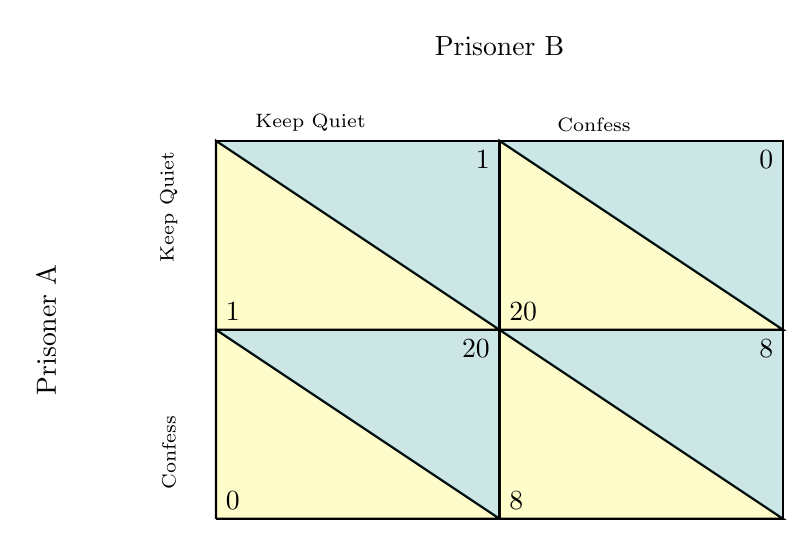
\begin{tikzpicture}[scale = 1.2]
%\draw[very thin, color = gray](0, 0) grid (12, 7);
\draw [thick, fill = yellow, fill opacity = 0.2] (3, 1) -- (6, 1) -- (3, 3) -- (3, 1);
\draw [thick, fill = teal, fill opacity = 0.2] (6, 1) -- (6, 3) -- (3, 3);
\draw [thick, fill = yellow, fill opacity = 0.2] (6, 1) -- (9, 1) -- (6, 3) -- (6, 1);
\draw [thick, fill = teal, fill opacity = 0.2] (9, 1) -- (9, 3) -- (6, 3);
\draw [thick, fill = yellow, fill opacity = 0.2] (6, 3) -- (9, 3) -- (6, 5) -- (6, 3);
\draw [thick, fill = teal, fill opacity = 0.2] (9, 3) -- (9, 5) -- (6, 5);
\draw [thick, fill = yellow, fill opacity = 0.2] (3, 3) -- (6, 3) -- (3, 5) -- (3, 3);
\draw [thick, fill = teal, fill opacity = 0.2] (6, 3) -- (6, 5) -- (3, 5);
\node at  (3, 1) [above right] {0};
\node at  (6, 3) [below left] {20};
\node at  (3, 3) [above right] {1};
\node at  (6, 5) [below left] {1};
\node at  (6, 1) [above right] {8};
\node at  (9, 3) [below left] {8};
\node at  (6, 3) [above right] {20};
\node at  (9, 5) [below left] {0};
\node at (4, 5) [above] {\scriptsize Keep Quiet};
\node at (7, 5) [above] {\scriptsize Confess};
\node [rotate = 90] at (2.5, 1.7) {\scriptsize Confess};
\node [rotate = 90] at (2.5, 4.3) {\scriptsize Keep Quiet};
\node at (6, 6) {Prisoner B};
\node [rotate = 90] at (1, 3) [below] {Prisoner A};
\end{tikzpicture}
\end{frame}

\begin{frame}{Prisoners' dilemma 2}
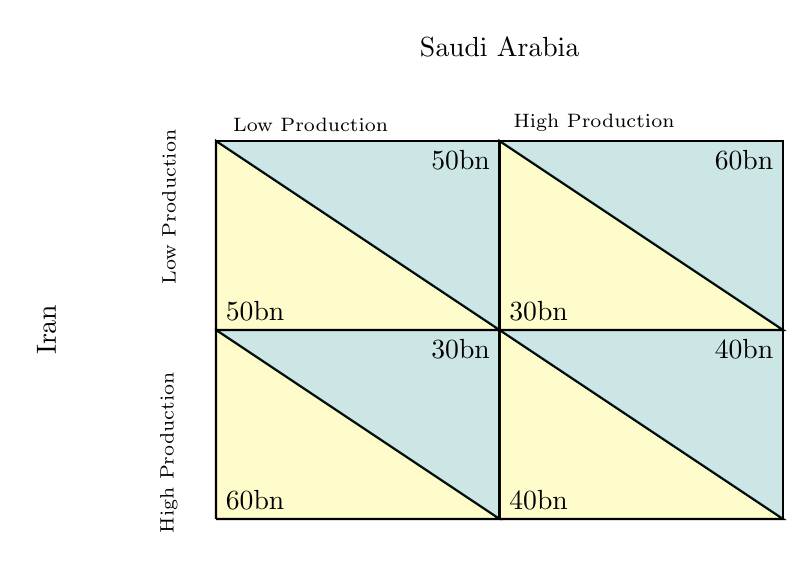
\begin{tikzpicture}[scale = 1.2]
%\draw[very thin, color = gray](0, 0) grid (12, 7);
\draw [thick, fill = yellow, fill opacity = 0.2] (3, 1) -- (6, 1) -- (3, 3) -- (3, 1);
\draw [thick, fill = teal, fill opacity = 0.2] (6, 1) -- (6, 3) -- (3, 3);
\draw [thick, fill = yellow, fill opacity = 0.2] (6, 1) -- (9, 1) -- (6, 3) -- (6, 1);
\draw [thick, fill = teal, fill opacity = 0.2] (9, 1) -- (9, 3) -- (6, 3);
\draw [thick, fill = yellow, fill opacity = 0.2] (6, 3) -- (9, 3) -- (6, 5) -- (6, 3);
\draw [thick, fill = teal, fill opacity = 0.2] (9, 3) -- (9, 5) -- (6, 5);
\draw [thick, fill = yellow, fill opacity = 0.2] (3, 3) -- (6, 3) -- (3, 5) -- (3, 3);
\draw [thick, fill = teal, fill opacity = 0.2] (6, 3) -- (6, 5) -- (3, 5);
\node at  (3, 1) [above right] {60bn};
\node at  (6, 3) [below left] {30bn};
\node at  (3, 3) [above right] {50bn};
\node at  (6, 5) [below left] {50bn};
\node at  (6, 1) [above right] {40bn};
\node at  (9, 3) [below left] {40bn};
\node at  (6, 3) [above right] {30bn};
\node at  (9, 5) [below left] {60bn};
\node at (4, 5) [above] {\scriptsize Low Production};
\node at (7, 5) [above] {\scriptsize High Production};
\node [rotate = 90] at (2.5, 1.7) {\scriptsize High Production};
\node [rotate = 90] at (2.5, 4.3) {\scriptsize Low Production};
\node at (6, 6) {Saudi Arabia};
\node [rotate = 90] at (1, 3) [below] {Iran};
\end{tikzpicture}
\end{frame}

\begin{frame}{Prisoners' dilemma 3}
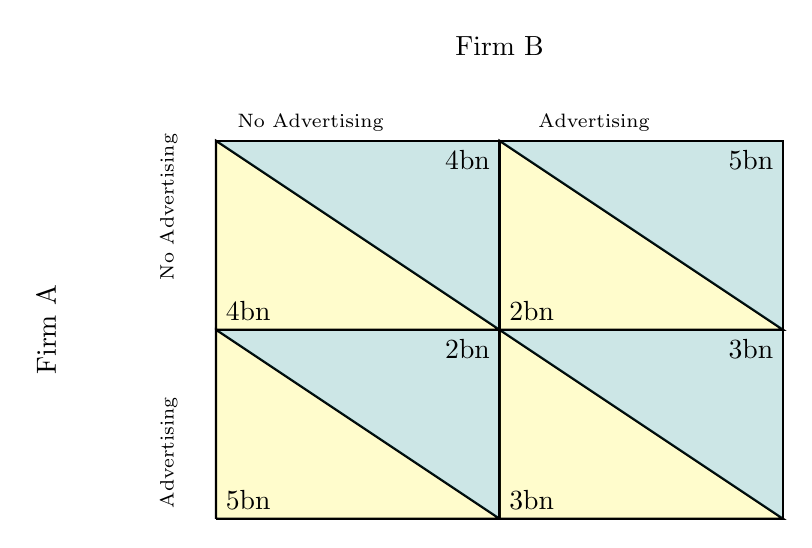
\begin{tikzpicture}[scale = 1.2]
%\draw[very thin, color = gray](0, 0) grid (12, 7);
\draw [thick, fill = yellow, fill opacity = 0.2] (3, 1) -- (6, 1) -- (3, 3) -- (3, 1);
\draw [thick, fill = teal, fill opacity = 0.2] (6, 1) -- (6, 3) -- (3, 3);
\draw [thick, fill = yellow, fill opacity = 0.2] (6, 1) -- (9, 1) -- (6, 3) -- (6, 1);
\draw [thick, fill = teal, fill opacity = 0.2] (9, 1) -- (9, 3) -- (6, 3);
\draw [thick, fill = yellow, fill opacity = 0.2] (6, 3) -- (9, 3) -- (6, 5) -- (6, 3);
\draw [thick, fill = teal, fill opacity = 0.2] (9, 3) -- (9, 5) -- (6, 5);
\draw [thick, fill = yellow, fill opacity = 0.2] (3, 3) -- (6, 3) -- (3, 5) -- (3, 3);
\draw [thick, fill = teal, fill opacity = 0.2] (6, 3) -- (6, 5) -- (3, 5);
\node at  (3, 1) [above right] {5bn};
\node at  (6, 3) [below left] {2bn};
\node at  (3, 3) [above right] {4bn};
\node at  (6, 5) [below left] {4bn};
\node at  (6, 1) [above right] {3bn};
\node at  (9, 3) [below left] {3bn};
\node at  (6, 3) [above right] {2bn};
\node at  (9, 5) [below left] {5bn};
\node at (4, 5) [above] {\scriptsize No Advertising};
\node at (7, 5) [above] {\scriptsize Advertising};
\node [rotate = 90] at (2.5, 1.7) {\scriptsize Advertising};
\node [rotate = 90] at (2.5, 4.3) {\scriptsize No Advertising};
\node at (6, 6) {Firm B};
\node [rotate = 90] at (1, 3) [below] {Firm A};
\end{tikzpicture}
\end{frame}

\begin{frame}{Cooperative games}
It is often the case that a better outcome can be reached with cooperation.  However, this demand some agreement between the parties. 
\pause
\begin{itemize}[<+-| alert@+>]
\item Commitment: taking some action that determines future decisions (\emph{Conquistadores})
\item Threats and punishment (Over-production, beating $\dots$)
\item Repeated games and \emph{Super-games}
\item The auction of G3 networks
\end{itemize}
\end{frame}




\section{Cournot, Bertrand and Stackleberg}
\begin{frame}{Models of Oligopoly}
Two firms facing a market demand curve can set quantity or price. 
\begin{itemize}[<+-| alert@+>]
\item \emph{Cournot model} Firms set output based on market demand and expected output of rival
\item \emph{residual demand} as the difference between market demand and the output of rival firm
\item \emph{Reaction function} is the output of firm A given the output of firm B
\item Nash equilibrium shows the optimal decision of each firm give the action of the rival
\end{itemize}
\end{frame}

\begin{frame}{Cournot model}
\begin{columns}[T]
\begin{column}{0.48\textwidth}
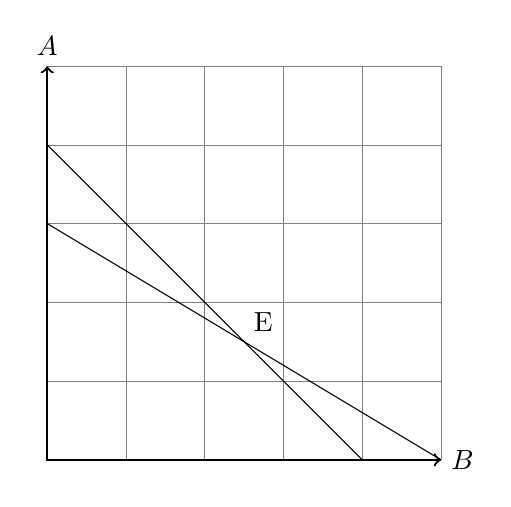
\begin{tikzpicture}
\draw [help lines] (0, 0) grid (5, 5);
\draw [<->, thick] (0, 5) node (yaxis) [above] {$A$} 
  |- (5, 0) node (xaxis) [right] {$B$};;
\draw (4, 0) -- (0, 4);
\draw (5, 0) --  (0, 3);
\node at (2.5, 1.5) [above right] {E};
\end{tikzpicture}
\end{column}
\begin{column}{.48\textwidth}
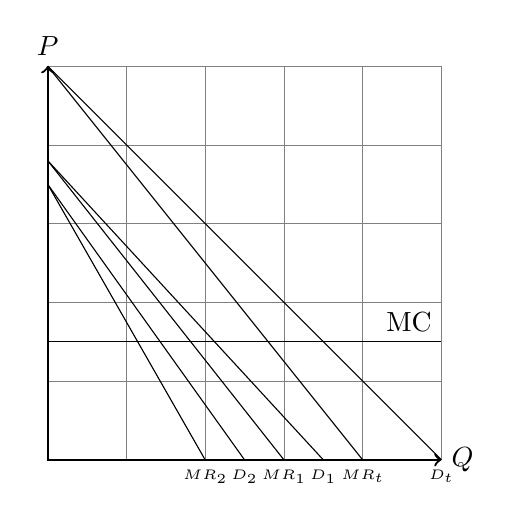
\begin{tikzpicture}
\draw[very thin, color = gray](0, 0) grid (5, 5);
\draw [<->, thick] (0, 5) node (yaxis) [above] {$P$} 
  |- (5, 0) node (xaxis) [right] {$Q$};
\draw (0, 5) to (5, 0);
\node at (5, 0) [below] {\tiny $D_t$};
\draw (0, 5) to (4, 0); 
\node at (4.0, 0) [below] {\tiny $MR_t$};
\draw (0, 3.8) to (3.5, 0);
\node at (3.5, 0) [below] {\tiny $D_1$};
\draw (0, 3.8) to (3, 0); 
\node at (3, 0) [below] {\tiny $MR_1$};
\draw (0, 3.5) to (2.5, 0);
\node at (2.5, 0) [below] {\tiny $D_2$};
\draw (0, 3.5) to (2, 0); 
\node at (2, 0) [below] {\tiny $MR_2$};
\draw (0, 1.5) -- (5, 1.5);
\node at (5, 1.5) [above left] {MC};
%\draw (0.25, 0.25) to (4.5, 3);
%\draw [dashed] (5, 1.70) to (0, 1.70);
%\draw[domain = 0.1:3.9, color = blue] plot(\x, {2 - 0.5*\x});
\end{tikzpicture}
\end{column}
\end{columns}
\end{frame}

\begin{frame}{Bertrand Model}
The two firms compete on price.  
\pause
\begin{itemize}[<+-| alert@+>]
\item If the first firm sets price above MC, the second can win market share by reducing the price
\item Competition will reduce the price towards the MC
\item MC is the Nash equilibrium
\end{itemize}
\end{frame}

\begin{frame}{Stackelberg Model}
Sequential moves  
\pause
\begin{itemize}[<+-| alert@+>]
\item One firm moves first (price or output)
\item There is \emph{first mover advantage}
\item Decision must consider what rival will do
\item Rival reacts to the credible announcement of the first mover
\item Issues
\begin{itemize}
\item Increased investment and output can lower costs through economies of scale
\item Increased costs will not be faced by rival
\end{itemize}
\end{itemize}
\end{frame}



\section{Controversies}
\begin{frame}{Controversies}
\begin{itemize}[<+-| alert@+>]
\item Retail price maintenance
\begin{itemize}
\item De Beers/Jeans 
\end{itemize}
\item Predatory pricing
\begin{itemize}
\item Lemon bus 
\end{itemize}
\item Tying
\begin{itemize}
\item Gillet-printers 
\end{itemize}

\end{itemize}
\end{frame}
%[<+-| alert@+>]




\end{document}
